% Pentest_report.tex
\documentclass[a4paper]{article}

\usepackage[utf8]{inputenc}
\usepackage[spanish]{babel}
\usepackage{graphicx} % Para la inserción de imagenes
\usepackage{lmodern}
\usepackage[dvipsnames,svgnames]{xcolor}
\usepackage[margin=2cm,top=2cm, includefoot]{geometry}
\usepackage[most]{tcolorbox}
\usepackage{fancyhdr}
\usepackage[hidelinks]{hyperref}
\usepackage{parskip}
\usepackage{listings}
\usepackage{smartdiagram}

% Declaración de colores
\definecolor{greenPortada}{RGB}{105,168,79}

% Declaración de variables
\newcommand{\logoPortada}{imagenes/logo.png} % Update this path to match your logo location
\newcommand{\logoMaquina}{imagenes/blue.png} % Update this path to match your machine logo location
\newcommand{\machineName}{Blue}

% Adicionales
% Ajuste de headheight recomendado por fancyhdr (evita el error "headheight is too small")
\setlength{\headheight}{60pt} % >= 54.67494pt sugerido por fancyhdr
\addtolength{\topmargin}{-14.47495pt} % opcional, sugerido por fancyhdr para mantener el diseño

\pagestyle{fancy}
\fancyhf{}
\lhead{\includegraphics[width=2.5cm]{\logoPortada}}\rhead{\includegraphics[width=1.5cm]{\logoMaquina}}
\renewcommand{\headrulewidth}{3pt}
\renewcommand{\headrule}{\hbox to\headwidth{%
    \color{greenPortada}\leaders\hrule height \headrulewidth\hfill}}

% Comienzo del documento
\begin{document}
        \cfoot{\thepage}
% Creacion de la portada
\begin{titlepage}
        \centering
        \includegraphics[width=0.6\textwidth]{\logoPortada}\par\vspace{1cm}
        {\LARGE \textbf{WRITE-UP}} \par\vspace{0.25cm}
        {\Huge\bfseries\textcolor{greenPortada}{Maquina \machineName}\par\vspace{1cm}}
        \vfill
        \includegraphics[width=\textwidth,height=9cm, keepaspectratio]{\logoMaquina}\par\vspace{0.5cm}
        \vfill
        \begin{tcolorbox}[colback=green!5!white,colframe=green!75!black]
        \centering
        {\Large Autor: Aarón Ibarra}\par\vspace{0.4cm}
        {\large Fecha: 31/Oct/2025}\par
        \end{tcolorbox}\par\vspace{0.1cm}
        \vfill
        {\large Todos los derechos reservados.}
        \vfill
        \end{titlepage}

        % Índice -------------------------------------------------------------------------------------
                \clearpage
        \tableofcontents
        \clearpage

        % Contenido del informe ----------------------------------------------------------------------
        % Introducción
        \section{Introducción}
        \vspace{0.2cm}

        \subsection{Antecedentes}
        La máquina {\textbf{\machineName}} de la plataforma \href{https://hackthebox.com}{\textbf{\textcolor{blue}{HackTheBox}}} es una de las más representativas para iniciarse en el pentesting de sistemas Windows. Su objetivo principal es exponer al atacante al análisis de servicios SMB y a la explotación de una vulnerabilidad crítica ampliamente conocida: MS17-010 (EternalBlue).
        \vspace{0.2cm}
        \begin{figure}[h]
                \centering
                
\includegraphics[width=0.55\textwidth]{imagenes/Blue details.png}
                \caption{Detalles de la máquina.}
        \end{figure}
        \vspace{0.2cm}
        \begin{tcolorbox}[enhanced,attach boxed title to top center={yshift=-3mm,yshifttext=-1mm},
                colback=blue!5!white,colframe=blue!75!black,colbacktitle=greenPortada!80!black,
                title=Dirección URL,fonttitle=\bfseries,
                boxed title style={size=small,colframe=blue!50!black} ]
                \centering
                \href{https://app.hackthebox.com/machines/blue}{\color{blue}{https://app.hackthebox.com/machines/blue}}
        \end{tcolorbox}
        \vspace{0.2cm}
        
        \subsection{Objetivos}
        Durante este ejercicio se busca desarrollar un flujo completo de ataque, desde la enumeración inicial hasta la obtención de una sesión privilegiada, comprendiendo cada etapa del proceso y reforzando la comprensión del impacto de vulnerabilidades no parcheadas en entornos reales.
        \vspace{0.5cm}
        \begin{figure}[h]
                \centering
                \smartdiagram[priority descriptive diagram]
                {Reconocimiento y enumeración de servicios SMB,
                Detección de vulnerabilidad \texttt{MS17-cd 10},
                Ejecución del exploit y obtención de shell}
                \caption{Fases del ataque.}
        \end{figure}
        \clearpage

        % Enumeración
        \section{Enumeración}
        \subsection{Reconocimiento inicial}
        Se comenzó realizando un analisis inicial sobre el sistema, verificando que el sistema objetivo se encontrara accesible desde nuestra máquina atacante. Para ello, se utilizó la herramienta \texttt{ping} para enviar paquetes ICMP al objetivo y confirmar su disponibilidad en la red. 
        \vspace{0.2cm}
        \begin{figure}[h]
                \centering
                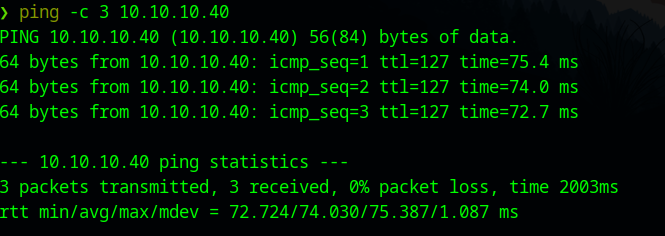
\includegraphics[width=0.7\textwidth]{../nmap/starting_recon.png}
                \caption{Reconocimiento inicial sobre el sistema objetivo.} 
        \end{figure}
        \vspace{0.2cm}
        
        Una vez localizado el sistema, se procedió a realizar un escaneo de puertos utilizando la herramienta \texttt{nmap} para identificar los servicios activos y sus versiones, obteniendo los siguientes resultados:
        \vspace{0.2cm}
        \begin{figure}[h]  
                \centering
                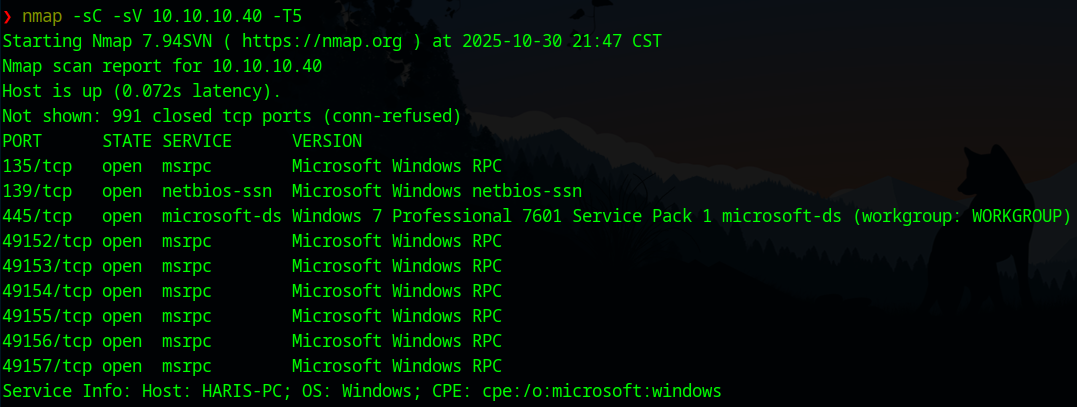
\includegraphics[width=.8\textwidth]{../nmap/nmap_initial.png}
                \caption{Escaneo inicial de puertos con nmap.}  
        \end{figure}
        \vspace{0.2cm}
        \subsection{Detección SMB}
        El módulo \texttt{auxiliary/scanner/smb/smb\_version} de Metasploit revela que el ovjetivo es vulnerable a la vulnerabilidad MS17-010, conocida como EternalBlue, que afecta a las versiones de Windows que utilizan el protocolo SMBv1.
        \vspace{0.2cm}
        \begin{figure}[h]
                \centering
                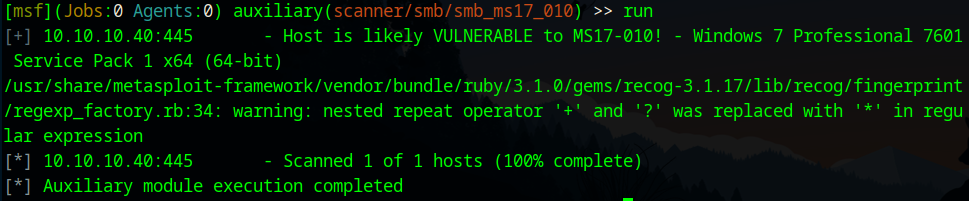
\includegraphics[width=.9\textwidth]{../nmap/smb.png}
                \caption{Detección de versión SMB con Metasploit.}
        \end{figure}
        \vspace{0.2cm}  
        \clearpage

        % Explotación
        \section{Explotación}
        Se verificó la vulnerabilidad MS17-010 \texttt{(EternalBlue)} en el servicio SMB del host 10.10.10.42 \texttt{(Windows 7 Professional SP1)}. \\ 
        Con el uso de Metasploit, se ejecutó el módulo \texttt{exploit/windows/smb/ms17\_010\_eternalblue} con el payload \texttt{windows/x64/shell\_reverse\_tcp}, lo que permitió abrir una sesión remota con privilegios de SYSTEM.
        \vspace{0.2cm}
        \begin{figure}[h]
                \centering
                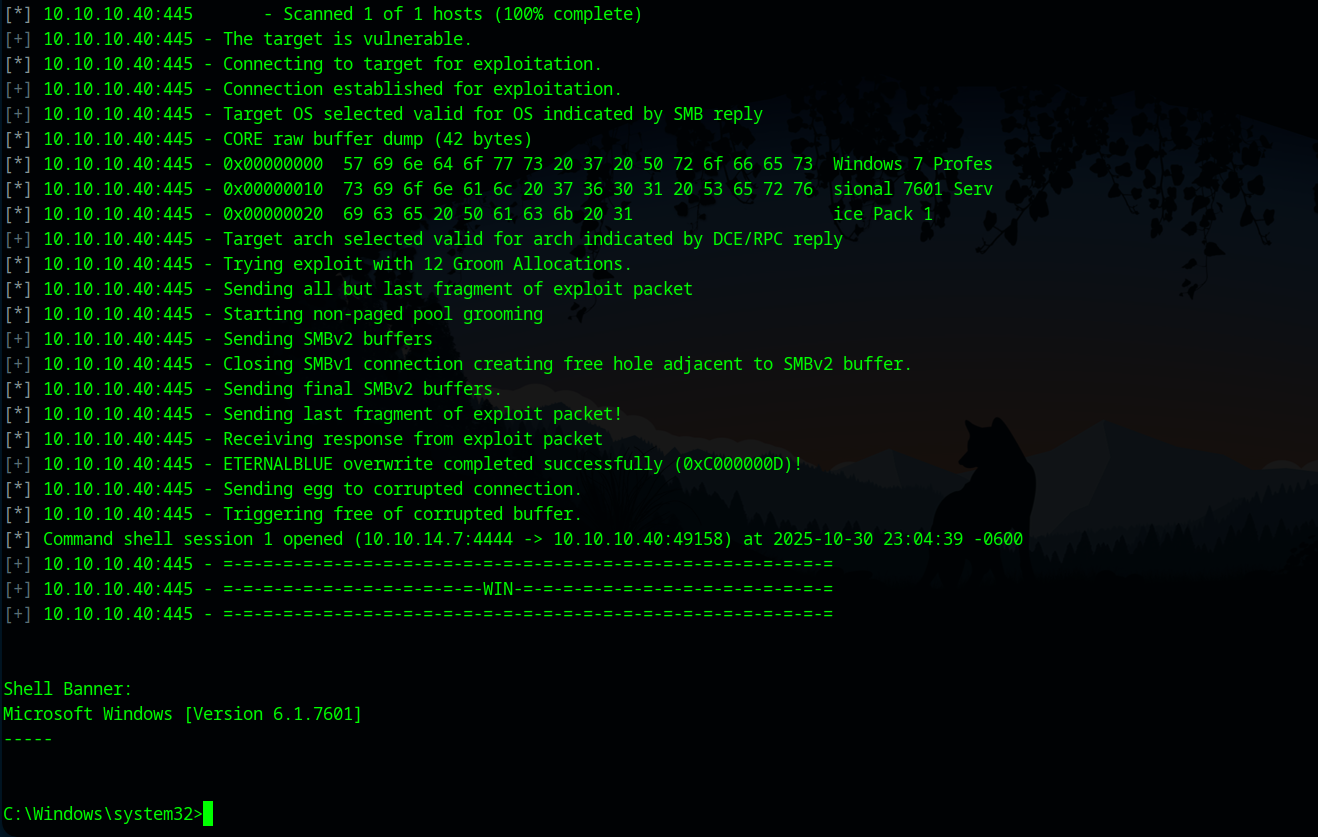
\includegraphics[width=.9\textwidth]{../exploits/shell.png}
                \caption{Explotación de la vulnerabilidad MS17-010 con Metasploit.}
        \end{figure}
        \vspace{0.2cm}

        \clearpage
        % Post-explotación
                \section{Post-explotación}
    Una vez obtenida la sesión remota, se recuperaron los archivos \verb|C:\Users\haris\Desktop\user.txt.txt| y \verb|C:\Users\Administrator\Desktop\root.txt.txt|.
        \vspace{0.2cm}
        \begin{figure}[h]
                \centering
                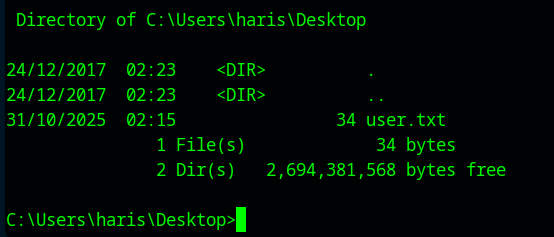
\includegraphics[width=.5\textwidth]{../exploits/user.png}
        \end{figure}
        \vspace{0.0005cm}
        \begin{figure}[h]
                \centering
                
\includegraphics[width=.5\textwidth]{../exploits/root.png}
                \caption{Obtención de la flags de usuario y root.}  
        \end{figure}
        \end{document}

